\documentclass{article}
\usepackage[utf8]{inputenc}
\usepackage{graphicx}
\usepackage{adjustbox}

\title{Website ER Diagram}
\date{October 2020}

% ------------
% DOCUMENT
% ------------
\begin{document}
    \begin{flushright}
        CSE 321 Website Storyboard
    \end{flushright}
    
    \begin{enumerate}
        \item[\textbf{Theme}:]
        Ice Breakr - A dating website that puts the conversation first.\\
    
        \item[\textbf{Group Name}:]
        Dream Machine\\
        Group #9\\
    
        \item[\textbf{Members}:]
        Logan Decker, Pierce Mayadag, Wesley Pick-Roth\\
    
        \item[\textbf{Background}:]
        When comparing the experiences of each members with websites and apps that we felt could use improvements, we determined that many dating sites tend to have similar problems that the conversations don't go anywhere, or that people feel shallow scrolling through and judging others based on their looks. So we decided to dedicate ourselves to creating a dating site that puts meaningful conversation and connection first, and people can gradually unlock additional interests and information as they talk more.\\
    
        \item[\textbf{Relevant Websites}]
            :Most standard dating websites require users to create a profile by filling out personal information which will then be used to match that user with another user that has related interests and characteristics.
            \begin{enumerate}
                \item[Tinder -]
                A quick and easy-to-use dating site with a focus on more immediate relationships and a minimal design.\\
                
                \item[Bumble -]
                A dating site where women make the first move. Focuses on user initiative by letting users choose the exact kind of relationship they want.\\
                
                \item[Hinge -]
                A dating site where the emphasis is on the user profiles. Tries to make long-lasting matches.\\
                
                \item[Plenty of Fish -]
                A typical dating site. Doesn't really try to focus in on anything.\\
                
                \item[OkCupid -]
                A dating site where matching is highly user-driven (users can look for very specific traits in partners).\\
            \end{enumerate}
        
        \item[\textbf{Desired Features}:]
        Users must 'unlock' information about a matching user by doing things like having a conversation in order to see user photos. Users will need to enter their location so as to try and match them with other users that are nearby. Users should be shown other potential matches one-at-a-time to try and avoid overloading the user with information. Users will need to enter the kind of relationship that they're looking for in order to better match them, for example, "looking for a short term relationship" or "looking for a lifelong partner". Users will need to fill out the answers to several questions in order to better match them, such as "What job do you have?" or "What do you like to do in your free time?". Our site will filter potential matches with user-specified age and distance filters, and, on the back end, match users with shared interests and information. Users will need to come up with topics of conversation or conversation starters that they find important so as to promote the initial conversation in a match.\\
    \end{enumerate}
    \hspace{-2cm}\begin{tabular}{|l|c|c|c|c|c|c|}
        \hline
         & IceBreakr & Tinder & Bumble & Hinge & Plenty of Fish & OkCupid \\
         \hline
         Location of Users & V- & X & X & X & X & X \\
         \hline
         Swipe-Matching & V & X & X & X & X & O \\
         \hline
         Relationship Categories & V & O & X+ & O & X & X+ \\
         \hline
         Personal Information Prompting & V & O & X & X & X & O \\
         \hline
         Unlocking Information & V+ & O & O & O & X & O \\
         \hline
         Filtering & V- & X & X+ & X+ & X & X+ \\
         \hline
         Interest Matching & V+ & X & O & O & X & X \\
         \hline
         Conversation Starters & V+ & X- & X & X & X & X \\
         \hline
    \end{tabular}
    X+: Function included well/focus placed on function\\
    X: Function included\\
    X-: Function included poorly/little focus placed on function\\
    O: Function not included\\
    V-: Function desired but not prioritized\\
    V: Function desired\\
    V+: Function desired and given priority\\
    
    \begin{enumerate}
        \item[\textbf{Potential Users}:]
        Registered users, unregistered users.\\
        
        \item[\textbf{User Stories & Storyboard}:]
        All users will start on the "home/login" page. The storyboard we've created is valid for all devices, as smaller screens (like phones) will display the same information in the same format, just with a smaller scaling. Unregistered users will be able to see a sample profile on the landing page to get an idea of what to expect from the website. From there, they can create an account where they'll fill out personal information. Once finished with account creation, they're redirected into the use-case scenario for registered users. For registered users, after logging in, they'll be taken to their own profile's page. Here, users can fill out additional information about themselves, or navigate to the "find matches" page or "messaging" page. Users may also manage their photos, which is its own page that allows users to upload, delete, and rearrange their photos. From any main page, users may navigate to their own profile, the messaging page, the matching page (all by using the buttons at the top of the page), and the landing page (by logging out). The "find matches" page will present the user with information about a different user and they will be prompted to accept or reject the match. The "messaging" page allows the user and any matches to message each other, as well as access the other users' profiles, which are identical to the personal profile except that some information is hidden until conversational benchmarks are met. The user storyboards are included in the "storyboard.pdf" file.
    \end{enumerate}
    
    \begin{enumerate}
        \item[\textbf{ER Diagram}:]
        The ER Diagram and the tables that follow are ways to visualize the way the database is going to be organized and implemented. We'll be able to look at the following information and easily determine what kinds of information we'll need to store and in what ways we'll be storing that information. We'll also be able to easily tell the relationships between the different objects in our system and how they interact.\\
        $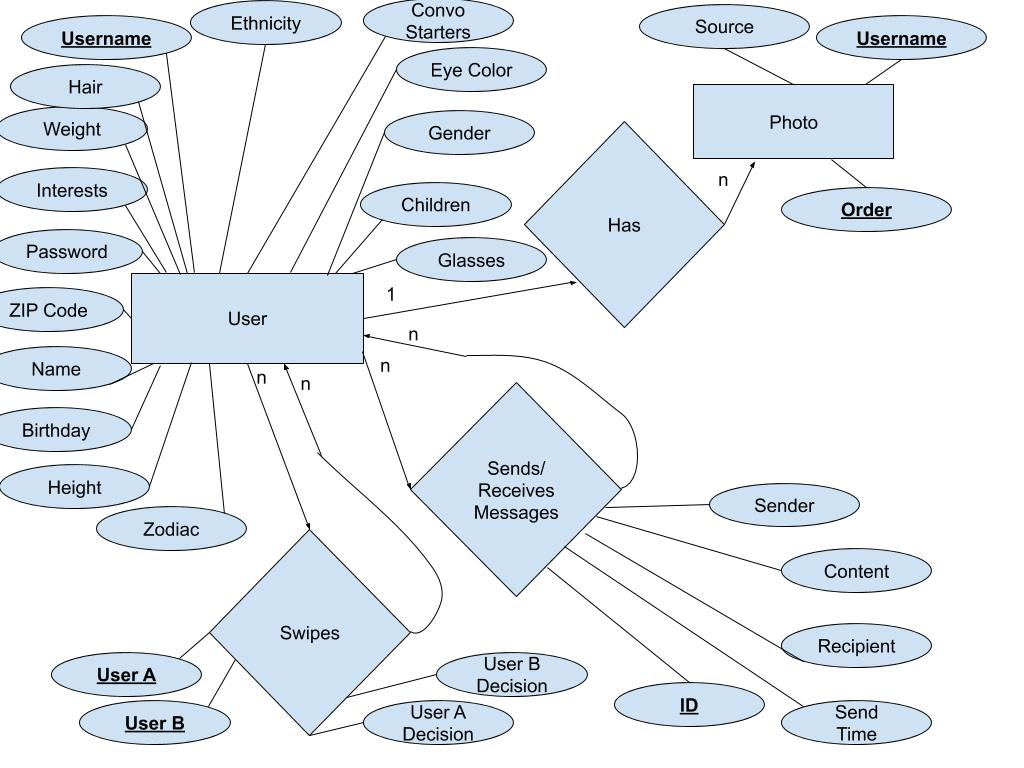
\includegraphics[width=0.9\columnwidth]{ERDiagram.jpg}$\\
        
        \item[\textbf{Table Design}:]
        \textbf{User Table}\\
        \begin{adjustbox}{width=1.2\textwidth}
            \begin{tabular}{|c|c|c|c|c|c|c|c|}
                \hline
                Primary Key & Field Name & Data Type & Non-Null & Unique & Binary & Foreign Key & Comments \\ \hline
                X & Username & varchar(32) & X & X &  & X & Identifies each user\\ \hline
                 & Password & varchar(32) & X &  &  &  & User's password\\ \hline
                 & Name & varchar(32) & X &  &  &  & User's real name\\ \hline
                 & Birthday & datetime & X &  &  &  & User's birth date\\ \hline
                 & Gender & uint(1) & X &  &  &  & User's gender (each value 0-9 corresponds to a list value)\\ \hline
                 & ZipCode & uint(5) & X &  &  &  & User's zip code\\ \hline
                 & HobbiesInterests & varchar(16) & X &  &  &  & Each bit corresponds to an interest (A 1 indicates an interest while a 0 indicates no interest)\\ \hline
                 & ConversationStarters & varchar(512) & X &  &  &  & Topics the user can talk about\\ \hline
                 & Height & uint(2) &  &  &  &  & User's total height in inches\\ \hline
                 & HairColor & uint(2) &  &  &  &  & User's hair color (each value 0-99 corresponds to a list value)\\ \hline
                 & ZodiacSign & uint(2) &  &  &  &  & User's zodiac sign (each value 0-99 corresponds to a list value)\\ \hline
                 & Children & uint(2) &  &  &  &  & Number of children the user has\\ \hline
                 & Weight & uint(3) &  &  &  &  & User's weight in pounds\\ \hline
                 & EyeColor & uint(1) &  &  &  &  & User's eye color (each value 0-9 corresponds to a list value)\\ \hline
                 & Ethnicity & varchar(32) &  &  &  &  & User's ethnicity\\ \hline
                 & Glasses & uint(1) &  &  & X &  & Whether or not the user wears glasses (0 if no, 1 if yes)\\ \hline
            \end{tabular}
        \end{adjustbox}\\
        This table holds all of the user's information. Each user has a unique username, and a password that they use to log into their account. They also have a lot of personal information. Most information is stored as a character string. The fields that aren't strings are stored as integers that correspond to values in lists. The idea is that users will select an option from a pre-determined list, and we store the position in that list. The hobbies/interests field is stored as a bit string, where each character in the string corresponds to a different hobby/interest. A 1 in that position indicates that the user has that hobby/interest, while a 0 indicates that the user does \textbf{not} have that hobby/interest. The date of the user's birth is stored as a datetime corresponding to midday of their birthday.\\
        The username must be unique, and, as such, is used for all other tables. By using the username as a foreign key, we can identify which user a Photo or Message belongs to, or whether or not they Swipe yay/nay on another user.\\
        
        \textbf{Photo Table}\\
        \begin{adjustbox}{width=1.2\textwidth}
            \begin{tabular}{|c|c|c|c|c|c|c|c|}
                \hline
                Primary Key & Field Name & Data Type & Non-Null & Unique & Binary & Foreign Key & Comments \\ \hline
                X & Username & varchar(32) & X & X &  & X & Identifies this photo's user\\ \hline
                X & Order & uint(1) & X & X &  &  & Determines position of this photo compared to others\\ \hline
                 & Source & varchar(256) &  &  &  &  & Photo's URL\\ \hline
            \end{tabular}
        \end{adjustbox}\\
        This table holds the information for a user's photos. Each user is allowed to have up to 9 photos. Each photo has a corresponding user and order (1-9) where a lower order means that it's displayed sooner. A value of 0 in the order means that the photo does not exist, which will occur if a user only has 8 or fewer photos. The source is the URL where the photo is uploaded. We'll use this URL to load the photo on our site.\\
        The username is used for all other tables. By using the username as a foreign key, we can identify which user these photos belong to.\\
        
        \textbf{Swipe Table}\\
        \begin{adjustbox}{width=1.2\textwidth}
            \begin{tabular}{|c|c|c|c|c|c|c|c|}
                \hline
                Primary Key & Field Name & Data Type & Non-Null & Unique & Binary & Foreign Key & Comments \\ \hline
                X & UserA & varchar(32) & X & X &  & X & Identifies first user of matching pair\\ \hline
                X & UserB & varchar(32) & X & X &  & X & Identifies second user of matching pair\\ \hline
                 & UserADecision & uint(1) &  &  & X &  & First user's swipe decision\\ \hline
                 & UserBDecision & uint(1) &  &  & X &  & Second user's swipe decision\\ \hline
            \end{tabular}
        \end{adjustbox}\\
        This table determines if two users are a match for each other. Each time a user swipes another user, if a table involving these two users doesn't already exist, a new one is created. The first user to swipe the other corresponds to UserA, and their decision is stored in UserADecision (0 if 'nay' and 1 if 'yay'). When the first user then shows up for the potential match, the second user and their decision are stored as UserB and UserBDecision. If both fields are 1s, it's a match! These two users may then start sending each other messages. While a user is undecided, their Decision field remains null.\\
        The two usernames are used to form the primary key for each match. Each username is a foreign key that corresponds to two different users that compose the match.\\
        
        \textbf{Message Table}\\
        \begin{adjustbox}{width=1.2\textwidth}
            \begin{tabular}{|c|c|c|c|c|c|c|c|}
                \hline
                Primary Key & Field Name & Data Type & Non-Null & Unique & Binary & Foreign Key & Comments \\ \hline
                X & ID & uint(8) & X & X &  &  & Identifies the specific message\\ \hline
                 & Sender & varchar(32) & X &  &  & X & Username of this message's sender\\ \hline
                 & Receiver & varchar(32) & X &  &  & X & Username of this message's recipient\\ \hline
                 & Content & varchar(512) & X &  &  &  & Content of the message\\ \hline
                 & TimeSent & datetime & X &  &  &  & Time at which this message was sent\\ \hline
            \end{tabular}
        \end{adjustbox}\\
        This table holds all the information for a message that one user sends to a matching user. The message ID is a unique 8-digit number that identifies this specific message. The sender and recipient are the users that this message is being sent between. The content contains the actual text of the message, and the time the message was sent is stored in TimeSent as a datetime. The TimeSent field will be used to sort the display of the messages.\\
        The two usernames are foreign keys that correspond to two different users that are messaging each other.\\
        
        \item[\textbf{System Architecture}:]
        $\includegraphics[width=0.9\columnwidth]{"SystemArchitecture.png"}$\\
        The User class stores all of a user's information (username, real name, gender, birthday, etc) as well as methods for getting and setting all of that data. It also contains some methods for generating special content, like Zodiac signs from the birthday.\\
        The Pictures class stores the URLs of all the photos of a user, as well as ways to get and set them. It also keeps track of how many photos the user has uploaded, which it updates using a special method.\\
        The Servlet file contains all of the logic for navigating between the pages as well as calls to the database for updating and receiving information. Depending on the action that it receives, it may load a new page, populate User and Pictures classes, update information in the database, pull information from the database, or more.\\
        The Profile, Other Profile, and Preview Profile jsp files display information from a User and a Pictures that the Servlet creates. The Profile file specifically also sends information to the Servlet for updating any user information, which updates the database. The Other Profile file check the User's Icebreakr Score before displaying some of the information. If the score isn't high enough, the information will be hidden. Increasing the score is done from the Servlet while sending messages. Preview Profile will never display fields that can be hidden and therefore doesn't ever use a Pictures class at all. Profile is accessed from Index, Conversation, Match, Other Profile, Pictures, and Signup. Other Profile is only accessed from Conversation. Preview Profile is accessed only from Index.\\
        The Pictures jsp file displays all photos that the logged-in user has (which are populated via the Servlet) and also sends updated URL information to the Servlet so that the Photo database can be updated. Pictures is only accessed from Profile.\\
    \end{enumerate}
\end{document}